%%%%% TITLE OF MAIN DOCUMENT %%%%%
%% NUMBER AND TITLE OF SECTION %%


%Some sample text to be displayed above the first subsection

%\subsection{Prinzip}

%Ein Zyklotron besteht aus Zwei hohlen, halbzylindrischen und Duanden an denen eine Spannung mit unterschiedlichem Vorzeichen anliegt, und darüber bzw. darunter liegende Magneten, die ein homogenes Magnetfeld erzeugen. Zudem gibt es einen Einlass und einen Auslass für Teilchen.

%\begin{wrapfigure}{r}{0.4\textwidth} \label{Zyklo}
%
%	\vspace{-10pt}
%	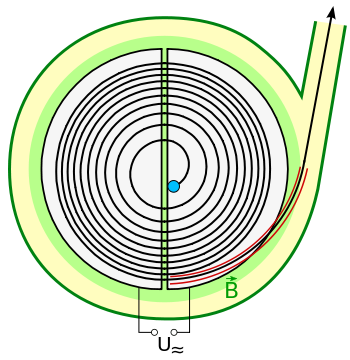
\includegraphics[width=0.35\textwidth]{Zyklotron_Prinzipskizze02.png}
%	\vspace{-13pt}
%	\caption{Prinzipskizze eines Zyklotrons}
%	\vspace{-5pt}	
%	
%\end{wrapfigure}

%\subsubsection{Anwendung}

% Some Formula:

%\begin{equation}
%	x= \frac{y \cdot 13 \pi z}
%			{\cos \alpha}
%\end{equation}

%%%%%%%%%%%%%%%%%%%%%%%
% Eigentlicher Beginn %
%%%%%%%%%%%%%%%%%%%%%%%


Da Elektronen negativ geladen sind (es \emph{sind} negative Ladungen), werden sie im elektrischen Feld zur positiven Seite hin beschleunigt, das heißt entgegen der Feldlinien. 

\subsection{Einwirkende Kraft}

Die Kraft ist abhängig von der Feldstärke und der Elektronenladung:

\begin{equation}
	F_{el} = E \cdot q_e
\end{equation}

\noindent Die Elektronenladung $q_e$ ist die konstante Ladung \emph{eines} Elektrons (\casio{23}). Zur experimentellen Bestimmung dieser, siehe \referenz{sec:Millikan}.

Im Kondensator gilt dann mit $E=\frac{U}{d}$:

\begin{equation} \label{eq:F_el}
	F_{el} = \frac{U}{d} \cdot q_e
\end{equation}
